% Options for packages loaded elsewhere
\PassOptionsToPackage{unicode}{hyperref}
\PassOptionsToPackage{hyphens}{url}
\PassOptionsToPackage{dvipsnames,svgnames,x11names}{xcolor}
%
\documentclass[
  letterpaper,
  DIV=11,
  numbers=noendperiod]{scrartcl}

\usepackage{amsmath,amssymb}
\usepackage{iftex}
\ifPDFTeX
  \usepackage[T1]{fontenc}
  \usepackage[utf8]{inputenc}
  \usepackage{textcomp} % provide euro and other symbols
\else % if luatex or xetex
  \usepackage{unicode-math}
  \defaultfontfeatures{Scale=MatchLowercase}
  \defaultfontfeatures[\rmfamily]{Ligatures=TeX,Scale=1}
\fi
\usepackage{lmodern}
\ifPDFTeX\else  
    % xetex/luatex font selection
\fi
% Use upquote if available, for straight quotes in verbatim environments
\IfFileExists{upquote.sty}{\usepackage{upquote}}{}
\IfFileExists{microtype.sty}{% use microtype if available
  \usepackage[]{microtype}
  \UseMicrotypeSet[protrusion]{basicmath} % disable protrusion for tt fonts
}{}
\makeatletter
\@ifundefined{KOMAClassName}{% if non-KOMA class
  \IfFileExists{parskip.sty}{%
    \usepackage{parskip}
  }{% else
    \setlength{\parindent}{0pt}
    \setlength{\parskip}{6pt plus 2pt minus 1pt}}
}{% if KOMA class
  \KOMAoptions{parskip=half}}
\makeatother
\usepackage{xcolor}
\setlength{\emergencystretch}{3em} % prevent overfull lines
\setcounter{secnumdepth}{-\maxdimen} % remove section numbering
% Make \paragraph and \subparagraph free-standing
\ifx\paragraph\undefined\else
  \let\oldparagraph\paragraph
  \renewcommand{\paragraph}[1]{\oldparagraph{#1}\mbox{}}
\fi
\ifx\subparagraph\undefined\else
  \let\oldsubparagraph\subparagraph
  \renewcommand{\subparagraph}[1]{\oldsubparagraph{#1}\mbox{}}
\fi

\usepackage{color}
\usepackage{fancyvrb}
\newcommand{\VerbBar}{|}
\newcommand{\VERB}{\Verb[commandchars=\\\{\}]}
\DefineVerbatimEnvironment{Highlighting}{Verbatim}{commandchars=\\\{\}}
% Add ',fontsize=\small' for more characters per line
\usepackage{framed}
\definecolor{shadecolor}{RGB}{241,243,245}
\newenvironment{Shaded}{\begin{snugshade}}{\end{snugshade}}
\newcommand{\AlertTok}[1]{\textcolor[rgb]{0.68,0.00,0.00}{#1}}
\newcommand{\AnnotationTok}[1]{\textcolor[rgb]{0.37,0.37,0.37}{#1}}
\newcommand{\AttributeTok}[1]{\textcolor[rgb]{0.40,0.45,0.13}{#1}}
\newcommand{\BaseNTok}[1]{\textcolor[rgb]{0.68,0.00,0.00}{#1}}
\newcommand{\BuiltInTok}[1]{\textcolor[rgb]{0.00,0.23,0.31}{#1}}
\newcommand{\CharTok}[1]{\textcolor[rgb]{0.13,0.47,0.30}{#1}}
\newcommand{\CommentTok}[1]{\textcolor[rgb]{0.37,0.37,0.37}{#1}}
\newcommand{\CommentVarTok}[1]{\textcolor[rgb]{0.37,0.37,0.37}{\textit{#1}}}
\newcommand{\ConstantTok}[1]{\textcolor[rgb]{0.56,0.35,0.01}{#1}}
\newcommand{\ControlFlowTok}[1]{\textcolor[rgb]{0.00,0.23,0.31}{#1}}
\newcommand{\DataTypeTok}[1]{\textcolor[rgb]{0.68,0.00,0.00}{#1}}
\newcommand{\DecValTok}[1]{\textcolor[rgb]{0.68,0.00,0.00}{#1}}
\newcommand{\DocumentationTok}[1]{\textcolor[rgb]{0.37,0.37,0.37}{\textit{#1}}}
\newcommand{\ErrorTok}[1]{\textcolor[rgb]{0.68,0.00,0.00}{#1}}
\newcommand{\ExtensionTok}[1]{\textcolor[rgb]{0.00,0.23,0.31}{#1}}
\newcommand{\FloatTok}[1]{\textcolor[rgb]{0.68,0.00,0.00}{#1}}
\newcommand{\FunctionTok}[1]{\textcolor[rgb]{0.28,0.35,0.67}{#1}}
\newcommand{\ImportTok}[1]{\textcolor[rgb]{0.00,0.46,0.62}{#1}}
\newcommand{\InformationTok}[1]{\textcolor[rgb]{0.37,0.37,0.37}{#1}}
\newcommand{\KeywordTok}[1]{\textcolor[rgb]{0.00,0.23,0.31}{#1}}
\newcommand{\NormalTok}[1]{\textcolor[rgb]{0.00,0.23,0.31}{#1}}
\newcommand{\OperatorTok}[1]{\textcolor[rgb]{0.37,0.37,0.37}{#1}}
\newcommand{\OtherTok}[1]{\textcolor[rgb]{0.00,0.23,0.31}{#1}}
\newcommand{\PreprocessorTok}[1]{\textcolor[rgb]{0.68,0.00,0.00}{#1}}
\newcommand{\RegionMarkerTok}[1]{\textcolor[rgb]{0.00,0.23,0.31}{#1}}
\newcommand{\SpecialCharTok}[1]{\textcolor[rgb]{0.37,0.37,0.37}{#1}}
\newcommand{\SpecialStringTok}[1]{\textcolor[rgb]{0.13,0.47,0.30}{#1}}
\newcommand{\StringTok}[1]{\textcolor[rgb]{0.13,0.47,0.30}{#1}}
\newcommand{\VariableTok}[1]{\textcolor[rgb]{0.07,0.07,0.07}{#1}}
\newcommand{\VerbatimStringTok}[1]{\textcolor[rgb]{0.13,0.47,0.30}{#1}}
\newcommand{\WarningTok}[1]{\textcolor[rgb]{0.37,0.37,0.37}{\textit{#1}}}

\providecommand{\tightlist}{%
  \setlength{\itemsep}{0pt}\setlength{\parskip}{0pt}}\usepackage{longtable,booktabs,array}
\usepackage{calc} % for calculating minipage widths
% Correct order of tables after \paragraph or \subparagraph
\usepackage{etoolbox}
\makeatletter
\patchcmd\longtable{\par}{\if@noskipsec\mbox{}\fi\par}{}{}
\makeatother
% Allow footnotes in longtable head/foot
\IfFileExists{footnotehyper.sty}{\usepackage{footnotehyper}}{\usepackage{footnote}}
\makesavenoteenv{longtable}
\usepackage{graphicx}
\makeatletter
\def\maxwidth{\ifdim\Gin@nat@width>\linewidth\linewidth\else\Gin@nat@width\fi}
\def\maxheight{\ifdim\Gin@nat@height>\textheight\textheight\else\Gin@nat@height\fi}
\makeatother
% Scale images if necessary, so that they will not overflow the page
% margins by default, and it is still possible to overwrite the defaults
% using explicit options in \includegraphics[width, height, ...]{}
\setkeys{Gin}{width=\maxwidth,height=\maxheight,keepaspectratio}
% Set default figure placement to htbp
\makeatletter
\def\fps@figure{htbp}
\makeatother

\usepackage{booktabs}
\usepackage{caption}
\usepackage{longtable}
\usepackage{colortbl}
\usepackage{array}
\usepackage{anyfontsize}
\usepackage{multirow}
\KOMAoption{captions}{tableheading}
\makeatletter
\@ifpackageloaded{caption}{}{\usepackage{caption}}
\AtBeginDocument{%
\ifdefined\contentsname
  \renewcommand*\contentsname{Table of contents}
\else
  \newcommand\contentsname{Table of contents}
\fi
\ifdefined\listfigurename
  \renewcommand*\listfigurename{List of Figures}
\else
  \newcommand\listfigurename{List of Figures}
\fi
\ifdefined\listtablename
  \renewcommand*\listtablename{List of Tables}
\else
  \newcommand\listtablename{List of Tables}
\fi
\ifdefined\figurename
  \renewcommand*\figurename{Figure}
\else
  \newcommand\figurename{Figure}
\fi
\ifdefined\tablename
  \renewcommand*\tablename{Table}
\else
  \newcommand\tablename{Table}
\fi
}
\@ifpackageloaded{float}{}{\usepackage{float}}
\floatstyle{ruled}
\@ifundefined{c@chapter}{\newfloat{codelisting}{h}{lop}}{\newfloat{codelisting}{h}{lop}[chapter]}
\floatname{codelisting}{Listing}
\newcommand*\listoflistings{\listof{codelisting}{List of Listings}}
\makeatother
\makeatletter
\makeatother
\makeatletter
\@ifpackageloaded{caption}{}{\usepackage{caption}}
\@ifpackageloaded{subcaption}{}{\usepackage{subcaption}}
\makeatother
\ifLuaTeX
  \usepackage{selnolig}  % disable illegal ligatures
\fi
\usepackage{bookmark}

\IfFileExists{xurl.sty}{\usepackage{xurl}}{} % add URL line breaks if available
\urlstyle{same} % disable monospaced font for URLs
\hypersetup{
  pdftitle={Final Project Exploratory Data Analysis},
  pdfauthor={Julia Vitale, Mia Zottoli, and Vishnu Lakshman},
  colorlinks=true,
  linkcolor={blue},
  filecolor={Maroon},
  citecolor={Blue},
  urlcolor={Blue},
  pdfcreator={LaTeX via pandoc}}

\title{Final Project Exploratory Data Analysis}
\author{Julia Vitale, Mia Zottoli, and Vishnu Lakshman}
\date{}

\begin{document}
\maketitle

\begin{Shaded}
\begin{Highlighting}[]
\CommentTok{\# Load necessary libraries}
\FunctionTok{library}\NormalTok{(here)}
\FunctionTok{library}\NormalTok{(tidyverse)}
\FunctionTok{library}\NormalTok{(ggplot2)}
\FunctionTok{library}\NormalTok{(corrr)}
\FunctionTok{library}\NormalTok{(ggcorrplot)}
\FunctionTok{library}\NormalTok{(FactoMineR)}
\FunctionTok{library}\NormalTok{(factoextra)}
\FunctionTok{library}\NormalTok{(ggfortify)}
\FunctionTok{library}\NormalTok{(cluster)}
\end{Highlighting}
\end{Shaded}

\begin{Shaded}
\begin{Highlighting}[]
\CommentTok{\# Load dataset}
\NormalTok{ultimate\_data }\OtherTok{\textless{}{-}} \FunctionTok{read\_csv}\NormalTok{(}\FunctionTok{here}\NormalTok{(}\StringTok{"data"}\NormalTok{, }\StringTok{"ultimate\_college\_championship.csv"}\NormalTok{)) }\SpecialCharTok{\%\textgreater{}\%}
\CommentTok{\# Standardise school names}
  \FunctionTok{mutate}\NormalTok{(}\FunctionTok{across}\NormalTok{(}\FunctionTok{c}\NormalTok{(level, gender, division, team\_name), as.factor)) }\SpecialCharTok{\%\textgreater{}\%}
  \FunctionTok{mutate}\NormalTok{(}\AttributeTok{school =} \FunctionTok{str\_split\_i}\NormalTok{(team\_name, }\StringTok{" "}\NormalTok{, }\DecValTok{1}\NormalTok{)) }\SpecialCharTok{\%\textgreater{}\%}
  \FunctionTok{mutate}\NormalTok{(}\AttributeTok{school =} \FunctionTok{ifelse}\NormalTok{(}\FunctionTok{str\_detect}\NormalTok{(team\_name, }\StringTok{"St Olaf"}\NormalTok{), }\StringTok{"St Olaf"}\NormalTok{, school)) }\SpecialCharTok{\%\textgreater{}\%}
  \FunctionTok{mutate}\NormalTok{(}\AttributeTok{school =} \FunctionTok{ifelse}\NormalTok{(}\FunctionTok{str\_detect}\NormalTok{(team\_name, }\StringTok{"North Carolina"}\NormalTok{), }\StringTok{"North Carolina"}\NormalTok{, school)) }\SpecialCharTok{\%\textgreater{}\%}
  \FunctionTok{mutate}\NormalTok{(}\AttributeTok{school =} \FunctionTok{ifelse}\NormalTok{(}\FunctionTok{str\_detect}\NormalTok{(team\_name, }\StringTok{"Cal Poly"}\NormalTok{), }\StringTok{"Cal Poly SLO"}\NormalTok{, school))  }\SpecialCharTok{\%\textgreater{}\%}
  \FunctionTok{mutate}\NormalTok{(}\AttributeTok{school =} \FunctionTok{ifelse}\NormalTok{(}\FunctionTok{str\_detect}\NormalTok{(team\_name, }\StringTok{"British Columbia"}\NormalTok{), }\StringTok{"British Columbia"}\NormalTok{, school))  }\SpecialCharTok{\%\textgreater{}\%}
  \FunctionTok{mutate}\NormalTok{(}\AttributeTok{school =} \FunctionTok{ifelse}\NormalTok{(}\FunctionTok{str\_detect}\NormalTok{(team\_name, }\StringTok{"Western Washington"}\NormalTok{), }\StringTok{"Western Washington"}\NormalTok{, school))  }\SpecialCharTok{\%\textgreater{}\%}
  \FunctionTok{mutate}\NormalTok{(}\AttributeTok{school =} \FunctionTok{ifelse}\NormalTok{(}\FunctionTok{str\_detect}\NormalTok{(team\_name, }\StringTok{"Penn State"}\NormalTok{), }\StringTok{"Penn State"}\NormalTok{, school))  }\SpecialCharTok{\%\textgreater{}\%}
  \FunctionTok{mutate}\NormalTok{(}\AttributeTok{school =} \FunctionTok{ifelse}\NormalTok{(}\FunctionTok{str\_detect}\NormalTok{(team\_name, }\StringTok{"San Diego"}\NormalTok{), }\StringTok{"UCSD"}\NormalTok{, school))  }\SpecialCharTok{\%\textgreater{}\%}
  \FunctionTok{mutate}\NormalTok{(}\AttributeTok{school =} \FunctionTok{ifelse}\NormalTok{(}\FunctionTok{str\_detect}\NormalTok{(team\_name, }\StringTok{"Lewis"}\NormalTok{), }\StringTok{"Lewis \& Clark"}\NormalTok{, school))  }\SpecialCharTok{\%\textgreater{}\%}
  \FunctionTok{mutate}\NormalTok{(}\AttributeTok{school =} \FunctionTok{ifelse}\NormalTok{(}\FunctionTok{str\_detect}\NormalTok{(team\_name, }\StringTok{"Colorado State"}\NormalTok{), }\StringTok{"Colorado State"}\NormalTok{, school))  }\SpecialCharTok{\%\textgreater{}\%}
  \FunctionTok{mutate}\NormalTok{(}\AttributeTok{school =} \FunctionTok{ifelse}\NormalTok{(}\FunctionTok{str\_detect}\NormalTok{(team\_name, }\StringTok{"Oklahoma Christian"}\NormalTok{), }\StringTok{"Oklahoma Christian"}\NormalTok{, school))  }\SpecialCharTok{\%\textgreater{}\%}
  \FunctionTok{mutate}\NormalTok{(}\AttributeTok{school =} \FunctionTok{ifelse}\NormalTok{(}\FunctionTok{str\_detect}\NormalTok{(team\_name, }\StringTok{"Binghamton"}\NormalTok{), }\StringTok{"SUNY Binghamton"}\NormalTok{, school))  }\SpecialCharTok{\%\textgreater{}\%}
  \FunctionTok{mutate}\NormalTok{(}\AttributeTok{school =} \FunctionTok{ifelse}\NormalTok{(}\FunctionTok{str\_detect}\NormalTok{(team\_name, }\StringTok{"Santa Bar"}\NormalTok{), }\StringTok{"UCSB"}\NormalTok{, school))  }\SpecialCharTok{\%\textgreater{}\%}
  \FunctionTok{mutate}\NormalTok{(}\AttributeTok{school =} \FunctionTok{ifelse}\NormalTok{(}\FunctionTok{str\_detect}\NormalTok{(team\_name, }\StringTok{"Santa Cr"}\NormalTok{), }\StringTok{"USCS"}\NormalTok{, school))  }\SpecialCharTok{\%\textgreater{}\%}
  \FunctionTok{mutate}\NormalTok{(}\AttributeTok{school =} \FunctionTok{ifelse}\NormalTok{(}\FunctionTok{str\_detect}\NormalTok{(team\_name, }\StringTok{"Colorado College"}\NormalTok{), }\StringTok{"Colorado College"}\NormalTok{, school))  }\SpecialCharTok{\%\textgreater{}\%}
  \FunctionTok{mutate}\NormalTok{(}\AttributeTok{school =} \FunctionTok{ifelse}\NormalTok{(}\FunctionTok{str\_detect}\NormalTok{(team\_name, }\StringTok{"Missouri S"}\NormalTok{), }\StringTok{"Missouri S\&T"}\NormalTok{, school))  }\SpecialCharTok{\%\textgreater{}\%}
  \FunctionTok{mutate}\NormalTok{(}\AttributeTok{school =} \FunctionTok{ifelse}\NormalTok{(}\FunctionTok{str\_detect}\NormalTok{(team\_name, }\StringTok{"Holyoke"}\NormalTok{), }\StringTok{"Mount Holyoke"}\NormalTok{, school))  }\SpecialCharTok{\%\textgreater{}\%}
  \FunctionTok{mutate}\NormalTok{(}\AttributeTok{school =} \FunctionTok{ifelse}\NormalTok{(}\FunctionTok{str\_detect}\NormalTok{(team\_name, }\StringTok{"NC State"}\NormalTok{), }\StringTok{"NC State"}\NormalTok{, school))  }\SpecialCharTok{\%\textgreater{}\%}
  \FunctionTok{mutate}\NormalTok{(}\AttributeTok{school =} \FunctionTok{ifelse}\NormalTok{(}\FunctionTok{str\_detect}\NormalTok{(team\_name, }\StringTok{"Oregon State"}\NormalTok{), }\StringTok{"Oregon State"}\NormalTok{, school))  }\SpecialCharTok{\%\textgreater{}\%}
  \FunctionTok{mutate}\NormalTok{(}\AttributeTok{school =} \FunctionTok{ifelse}\NormalTok{(}\FunctionTok{str\_detect}\NormalTok{(team\_name, }\StringTok{"Washington University"}\NormalTok{), }\StringTok{"Washington University"}\NormalTok{, school))}
\end{Highlighting}
\end{Shaded}

\subsection{Exploring the Data}\label{exploring-the-data}

Answer the following questions:

\begin{itemize}
\tightlist
\item
  What is your outcome variable(s)? How well does it measure the outcome
  you are interested? How does it relate to your expectations?
\end{itemize}

\emph{Our outcome variable is plus\_minus, which is the difference
between the amount of points scored by an individual player's team while
that player is on the field and the amount of points scored by the
opposing team while that player is on the field. We are interested in
the influence of an individual player on the success of the whole team,
so this variable is a good measure of our outcome of interest.}

\emph{Essentially, +/- for a select player = points scored by player's
team (while player is on the field) - points scored by opposing team
(while player is on the field)}

\emph{The +/- score is used to track a player's overall effectiveness on
the field and their impact on the game. A positive +/- score means the
player's team scored more than the opposing team while the player was on
the field, and a negative +/- score means the opposing team scored more
while the player was on the field.}

\begin{itemize}
\item
  What are your key explanatory variables?

  \emph{Turns (turnovers) thrown per game, points scored per game, Ds
  (defensive interceptions) per game, assists per game, level (Division
  1 or 3), division (Men's or Women's) and school.}
\end{itemize}

In addition, create a table of summary statistics for the variables you
are planning to use.

\begin{Shaded}
\begin{Highlighting}[]
\CommentTok{\# A table of summarizing statistics of the variables we are planning to use }
\NormalTok{ultimate\_data }\SpecialCharTok{\%\textgreater{}\%} \FunctionTok{select}\NormalTok{(}\SpecialCharTok{{-}}\FunctionTok{c}\NormalTok{(player, team\_name)) }\SpecialCharTok{\%\textgreater{}\%}\NormalTok{ gtsummary}\SpecialCharTok{::}\FunctionTok{tbl\_summary}\NormalTok{()}
\end{Highlighting}
\end{Shaded}

\begin{table}
\fontsize{12.0pt}{14.4pt}\selectfont
\begin{tabular*}{\linewidth}{@{\extracolsep{\fill}}lc}
\toprule
\textbf{Characteristic} & \textbf{N = 1,665}\textsuperscript{\textit{1}} \\ 
\midrule\addlinespace[2.5pt]
level &  \\ 
    Division 1 & 973 (58\%) \\ 
    Division 3 & 692 (42\%) \\ 
gender &  \\ 
    Men & 893 (54\%) \\ 
    Women & 772 (46\%) \\ 
division &  \\ 
    Division 1 Men & 521 (31\%) \\ 
    Division 1 Women & 452 (27\%) \\ 
    Division 3 Men & 372 (22\%) \\ 
    Division 3 Women & 320 (19\%) \\ 
Turns & 2 (0, 7) \\ 
Ds & 1.00 (0.00, 3.00) \\ 
Assists & 1.0 (0.0, 3.0) \\ 
Points & 1.0 (0.0, 4.0) \\ 
plus\_minus & 1 (0, 5) \\ 
team\_games &  \\ 
    5 & 780 (47\%) \\ 
    6 & 738 (44\%) \\ 
    7 & 122 (7.3\%) \\ 
    8 & 25 (1.5\%) \\ 
turns\_per\_game & 0.40 (0.00, 1.17) \\ 
ds\_per\_game & 0.20 (0.00, 0.50) \\ 
ast\_per\_game & 0.17 (0.00, 0.60) \\ 
pts\_per\_game & 0.20 (0.00, 0.71) \\ 
pls\_mns\_per\_game & 0.20 (0.00, 0.83) \\ 
school &  \\ 
    Alabama-Huntsville & 23 (1.4\%) \\ 
    Bates & 17 (1.0\%) \\ 
    Berry & 26 (1.6\%) \\ 
    British Columbia & 23 (1.4\%) \\ 
    Brown & 25 (1.5\%) \\ 
    Cal & 23 (1.4\%) \\ 
    Cal Poly SLO & 24 (1.4\%) \\ 
    Carleton & 101 (6.1\%) \\ 
    Claremont & 24 (1.4\%) \\ 
    Colorado & 49 (2.9\%) \\ 
    Colorado College & 22 (1.3\%) \\ 
    Colorado State & 21 (1.3\%) \\ 
    Davenport & 31 (1.9\%) \\ 
    Franciscan & 22 (1.3\%) \\ 
    Georgia & 45 (2.7\%) \\ 
    Grinnell & 15 (0.9\%) \\ 
    Haverford/Bryn & 24 (1.4\%) \\ 
    Lewis \& Clark & 44 (2.6\%) \\ 
    Macalester & 20 (1.2\%) \\ 
    Massachusetts & 28 (1.7\%) \\ 
    Michigan & 54 (3.2\%) \\ 
    Middlebury & 53 (3.2\%) \\ 
    Minnesota & 28 (1.7\%) \\ 
    Missouri S\&T & 15 (0.9\%) \\ 
    Mount Holyoke & 12 (0.7\%) \\ 
    NC State & 30 (1.8\%) \\ 
    North Carolina & 61 (3.7\%) \\ 
    Oberlin & 22 (1.3\%) \\ 
    Occidental & 23 (1.4\%) \\ 
    Oklahoma Christian & 24 (1.4\%) \\ 
    Oregon & 51 (3.1\%) \\ 
    Oregon State & 22 (1.3\%) \\ 
    Ottawa & 16 (1.0\%) \\ 
    Penn State & 24 (1.4\%) \\ 
    Pennsylvania & 22 (1.3\%) \\ 
    Pittsburgh & 28 (1.7\%) \\ 
    Portland & 24 (1.4\%) \\ 
    Richmond & 39 (2.3\%) \\ 
    Rochester & 25 (1.5\%) \\ 
    St Olaf & 51 (3.1\%) \\ 
    Stanford & 22 (1.3\%) \\ 
    SUNY Binghamton & 22 (1.3\%) \\ 
    Texas & 26 (1.6\%) \\ 
    Tufts & 21 (1.3\%) \\ 
    UCSB & 23 (1.4\%) \\ 
    UCSD & 25 (1.5\%) \\ 
    Union & 18 (1.1\%) \\ 
    USCS & 21 (1.3\%) \\ 
    Utah & 22 (1.3\%) \\ 
    Vermont & 46 (2.8\%) \\ 
    Victoria & 20 (1.2\%) \\ 
    Washington & 26 (1.6\%) \\ 
    Washington University & 29 (1.7\%) \\ 
    Wellesley & 20 (1.2\%) \\ 
    Wesleyan & 22 (1.3\%) \\ 
    Western Washington & 23 (1.4\%) \\ 
    Whitman & 22 (1.3\%) \\ 
    Williams & 26 (1.6\%) \\ 
\bottomrule
\end{tabular*}
\begin{minipage}{\linewidth}
\textsuperscript{\textit{1}}n (\%); Median (Q1, Q3)\\
\end{minipage}
\end{table}

\subsection{Data Wrangling and
Transformation}\label{data-wrangling-and-transformation}

Answer the following question:

\begin{itemize}
\item
  What data cleaning did you have to do?

  \begin{itemize}
  \tightlist
  \item
    \textbf{The data was already pretty clean. We had to do some string
    manipulation to extract the school name from the team name, and had
    to convert some character variables to factors.}
  \end{itemize}
\item
  How did you wrangle the data?

  \begin{itemize}
  \tightlist
  \item
    \textbf{We did not have to do significant data wrangling for this
    data set. If we choose an analysis method that requires
    standardization, we will have to standardize the numeric variables.}
  \end{itemize}
\item
  Are you deciding to exclude any observations? If so, why?

  \begin{itemize}
  \tightlist
  \item
    \textbf{No, we are not excluding any observations. There are no
    extreme outliers.}
  \end{itemize}
\item
  Did you have to create any new variables from existing variables? If
  so, how and why?

  \begin{itemize}
  \tightlist
  \item
    \textbf{We created a `school' variable which extracts the name of
    the college/university associated with the team name. Some schools
    have both men's and women's teams in this data set, and we are
    curious if school advantage transcends team-specific advantage.}
  \end{itemize}
\end{itemize}

\subsection{Codebook}\label{codebook}

We have created a codebook in the README.md page in our repo on GitHub
which contains a description of all the variables we are using.

You must add a \emph{codebook} -- a description of all variables you are
using, including ones you are creating for this project -- to the
README.md page of the \texttt{data/} folder of your repo.

\subsection{Data Visualization}\label{data-visualization}

We have 11 data visualizations of our data made in R. Our outcome
variable, which is \texttt{plus\_minus}, is used in multiple
visualizations. There are visualizations involving various different
data types (categorical, numerical, continuous and discrete).

\begin{Shaded}
\begin{Highlighting}[]
\CommentTok{\# Plot player\textquotesingle{}s plus{-}minus scores and their gender}
\FunctionTok{ggplot}\NormalTok{(ultimate\_data, }\FunctionTok{aes}\NormalTok{(}\AttributeTok{x =}\NormalTok{ gender, }\AttributeTok{y =}\NormalTok{ plus\_minus, }\AttributeTok{fill =}\NormalTok{ gender)) }\SpecialCharTok{+}
  \FunctionTok{geom\_boxplot}\NormalTok{() }\SpecialCharTok{+}
  \FunctionTok{labs}\NormalTok{(}
    \AttributeTok{title =} \StringTok{"Gender vs. Player\textquotesingle{}s +/{-} Score"}\NormalTok{,}
    \AttributeTok{x =} \StringTok{"Gender"}\NormalTok{,}
    \AttributeTok{y =} \StringTok{"Player\textquotesingle{}s +/{-} Score"}
\NormalTok{  ) }\SpecialCharTok{+}
  \FunctionTok{theme\_minimal}\NormalTok{()}
\end{Highlighting}
\end{Shaded}

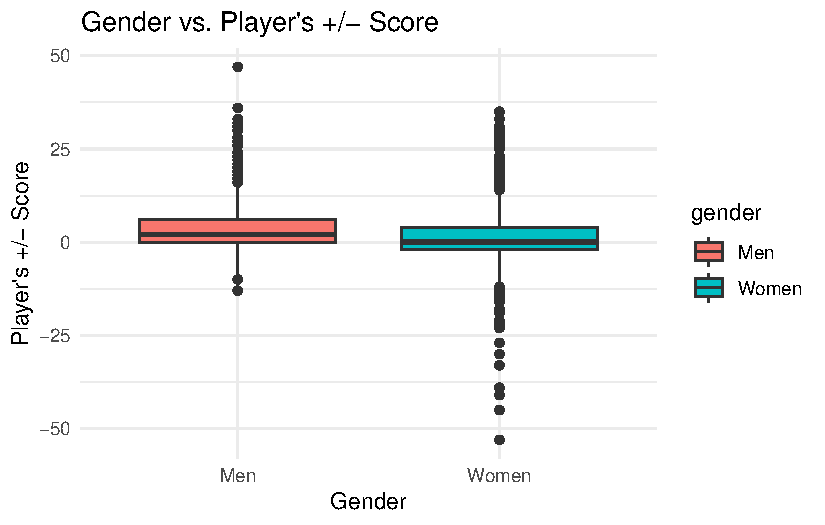
\includegraphics{final_eda_files/figure-pdf/gender-&-plus-minus-1.pdf}

\begin{Shaded}
\begin{Highlighting}[]
\CommentTok{\# Filter table to create a new table called d3 that only contains d3 level players}
\NormalTok{d3 }\OtherTok{\textless{}{-}}\NormalTok{ ultimate\_dataset[ultimate\_dataset}\SpecialCharTok{$}\NormalTok{level }\SpecialCharTok{==} \StringTok{"Division 3"}\NormalTok{,]}
\end{Highlighting}
\end{Shaded}

\begin{verbatim}
Error in eval(expr, envir, enclos): object 'ultimate_dataset' not found
\end{verbatim}

\begin{Shaded}
\begin{Highlighting}[]
\CommentTok{\# Plot  Division 3 level player\textquotesingle{}s plus{-}minus scores and their gender}
\FunctionTok{ggplot}\NormalTok{(d3, }\FunctionTok{aes}\NormalTok{(}\AttributeTok{x =}\NormalTok{ gender, }\AttributeTok{y =}\NormalTok{ plus\_minus, }\AttributeTok{fill =}\NormalTok{ gender)) }\SpecialCharTok{+}
  \FunctionTok{geom\_boxplot}\NormalTok{() }\SpecialCharTok{+}
  \FunctionTok{labs}\NormalTok{(}
    \AttributeTok{title =} \StringTok{"Division 3 Gender vs. Player\textquotesingle{}s +/{-} Score"}\NormalTok{,}
    \AttributeTok{x =} \StringTok{"Gender"}\NormalTok{,}
    \AttributeTok{y =} \StringTok{"Player\textquotesingle{}s +/{-} Score"}
\NormalTok{  ) }\SpecialCharTok{+}
  \FunctionTok{theme\_minimal}\NormalTok{()}
\end{Highlighting}
\end{Shaded}

\begin{verbatim}
Error in eval(expr, envir, enclos): object 'd3' not found
\end{verbatim}

\begin{Shaded}
\begin{Highlighting}[]
\CommentTok{\# Filter table to create a new table called d1 that only contains d3 level players}
\NormalTok{d1 }\OtherTok{\textless{}{-}}\NormalTok{ ultimate\_dataset[ultimate\_dataset}\SpecialCharTok{$}\NormalTok{level }\SpecialCharTok{==} \StringTok{"Division 1"}\NormalTok{,]}
\end{Highlighting}
\end{Shaded}

\begin{verbatim}
Error in eval(expr, envir, enclos): object 'ultimate_dataset' not found
\end{verbatim}

\begin{Shaded}
\begin{Highlighting}[]
\CommentTok{\# Plot  Division 1 level player\textquotesingle{}s plus{-}minus scores and their gender}
\FunctionTok{ggplot}\NormalTok{(d1, }\FunctionTok{aes}\NormalTok{(}\AttributeTok{x =}\NormalTok{ gender, }\AttributeTok{y =}\NormalTok{ plus\_minus, }\AttributeTok{fill =}\NormalTok{ gender)) }\SpecialCharTok{+}
  \FunctionTok{geom\_boxplot}\NormalTok{() }\SpecialCharTok{+}
  \FunctionTok{labs}\NormalTok{(}
    \AttributeTok{title =} \StringTok{"Division 1 Gender vs. Player\textquotesingle{}s +/{-} Score"}\NormalTok{,}
    \AttributeTok{x =} \StringTok{"Gender"}\NormalTok{,}
    \AttributeTok{y =} \StringTok{"Player\textquotesingle{}s +/{-} Score"}
\NormalTok{  ) }\SpecialCharTok{+}
  \FunctionTok{theme\_minimal}\NormalTok{()}
\end{Highlighting}
\end{Shaded}

\begin{verbatim}
Error in eval(expr, envir, enclos): object 'd1' not found
\end{verbatim}

\begin{Shaded}
\begin{Highlighting}[]
\CommentTok{\# Plot player\textquotesingle{}s plus{-}minus score against the divisional level they are playing in}
\FunctionTok{ggplot}\NormalTok{(ultimate\_data, }\FunctionTok{aes}\NormalTok{(}\AttributeTok{x =}\NormalTok{ level, }\AttributeTok{y =}\NormalTok{ plus\_minus, }\AttributeTok{fill =}\NormalTok{ level)) }\SpecialCharTok{+}
  \FunctionTok{geom\_violin}\NormalTok{(}\AttributeTok{trim =} \ConstantTok{FALSE}\NormalTok{) }\SpecialCharTok{+}
  \FunctionTok{labs}\NormalTok{(}
    \AttributeTok{title =} \StringTok{"Player\textquotesingle{}s +/{-} Score for Division 1 vs Division 3"}\NormalTok{,}
    \AttributeTok{x =} \StringTok{"Division"}\NormalTok{,}
    \AttributeTok{y =} \StringTok{"Player\textquotesingle{}s +/{-} Score"}
\NormalTok{  ) }\SpecialCharTok{+}
  \FunctionTok{scale\_fill\_manual}\NormalTok{(}\AttributeTok{values =} \FunctionTok{c}\NormalTok{(}\StringTok{"Division 1"} \OtherTok{=} \StringTok{"blue"}\NormalTok{, }\StringTok{"Division 3"} \OtherTok{=} \StringTok{"pink"}\NormalTok{)) }\SpecialCharTok{+} 
  \FunctionTok{theme\_minimal}\NormalTok{()}
\end{Highlighting}
\end{Shaded}

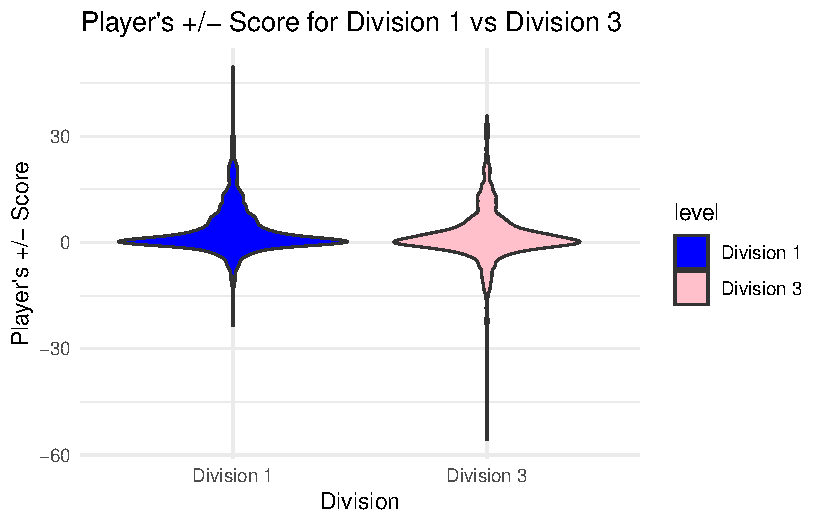
\includegraphics{final_eda_files/figure-pdf/division-level-&-plus-minus-1.pdf}

\begin{Shaded}
\begin{Highlighting}[]
\CommentTok{\# Filter table to create a new table called women\_ultimate\_data that only contains female players}
\NormalTok{women\_ultimate\_data }\OtherTok{\textless{}{-}}\NormalTok{ ultimate\_data }\SpecialCharTok{\%\textgreater{}\%}
  \FunctionTok{filter}\NormalTok{(gender }\SpecialCharTok{==} \StringTok{"Women"}\NormalTok{)}

\CommentTok{\# Plot female player\textquotesingle{}s plus{-}minus score against the divisional level they are playing in}
\FunctionTok{ggplot}\NormalTok{(women\_ultimate\_data, }\FunctionTok{aes}\NormalTok{(}\AttributeTok{x =}\NormalTok{ level, }\AttributeTok{y =}\NormalTok{ plus\_minus, }\AttributeTok{fill =}\NormalTok{ level)) }\SpecialCharTok{+}
  \FunctionTok{geom\_violin}\NormalTok{(}\AttributeTok{trim =} \ConstantTok{FALSE}\NormalTok{) }\SpecialCharTok{+}
  \FunctionTok{labs}\NormalTok{(}
    \AttributeTok{title =} \StringTok{"Player\textquotesingle{}s +/{-} Score for Division 1 vs Division 3 Women"}\NormalTok{,}
    \AttributeTok{x =} \StringTok{"Division"}\NormalTok{,}
    \AttributeTok{y =} \StringTok{"Player\textquotesingle{}s +/{-} Score"}
\NormalTok{  ) }\SpecialCharTok{+}
  \FunctionTok{scale\_fill\_manual}\NormalTok{(}\AttributeTok{values =} \FunctionTok{c}\NormalTok{(}\StringTok{"Division 1"} \OtherTok{=} \StringTok{"blue"}\NormalTok{, }\StringTok{"Division 3"} \OtherTok{=} \StringTok{"pink"}\NormalTok{)) }\SpecialCharTok{+} 
  \FunctionTok{theme\_minimal}\NormalTok{()}
\end{Highlighting}
\end{Shaded}

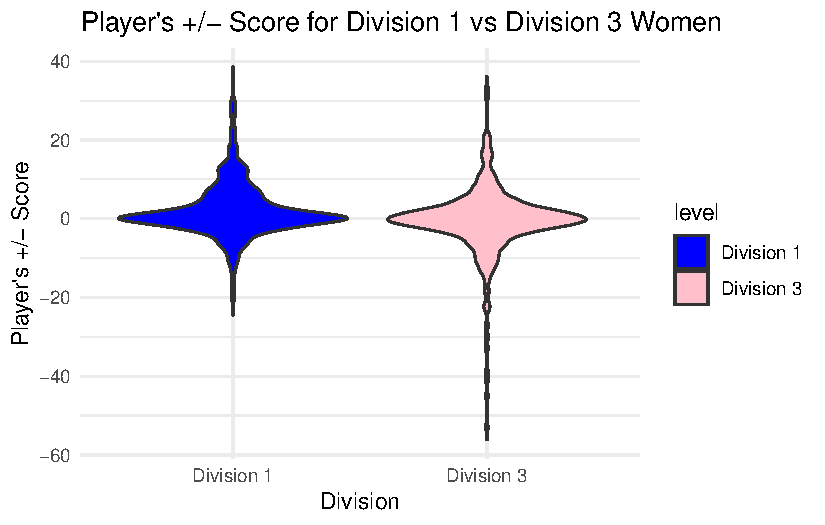
\includegraphics{final_eda_files/figure-pdf/division-level-&-plus-minus-2.pdf}

\begin{Shaded}
\begin{Highlighting}[]
\CommentTok{\# Filter table to create a new table called men\_ultimate\_data that only contains male players}
\NormalTok{men\_ultimate\_data }\OtherTok{\textless{}{-}}\NormalTok{ ultimate\_data }\SpecialCharTok{\%\textgreater{}\%}
  \FunctionTok{filter}\NormalTok{(gender }\SpecialCharTok{==} \StringTok{"Men"}\NormalTok{)}

\CommentTok{\# Plot male player\textquotesingle{}s plus{-}minus score against the divisional level they are playing in}
\FunctionTok{ggplot}\NormalTok{(men\_ultimate\_data, }\FunctionTok{aes}\NormalTok{(}\AttributeTok{x =}\NormalTok{ level, }\AttributeTok{y =}\NormalTok{ plus\_minus, }\AttributeTok{fill =}\NormalTok{ level)) }\SpecialCharTok{+}
  \FunctionTok{geom\_violin}\NormalTok{(}\AttributeTok{trim =} \ConstantTok{FALSE}\NormalTok{) }\SpecialCharTok{+}
  \FunctionTok{labs}\NormalTok{(}
    \AttributeTok{title =} \StringTok{"Player\textquotesingle{}s +/{-} Score for Division 1 vs Division 3 Men"}\NormalTok{,}
    \AttributeTok{x =} \StringTok{"Division"}\NormalTok{,}
    \AttributeTok{y =} \StringTok{"Player\textquotesingle{}s +/{-} Score"}
\NormalTok{  ) }\SpecialCharTok{+}
  \FunctionTok{scale\_fill\_manual}\NormalTok{(}\AttributeTok{values =} \FunctionTok{c}\NormalTok{(}\StringTok{"Division 1"} \OtherTok{=} \StringTok{"blue"}\NormalTok{, }\StringTok{"Division 3"} \OtherTok{=} \StringTok{"pink"}\NormalTok{)) }\SpecialCharTok{+} 
  \FunctionTok{theme\_minimal}\NormalTok{()}
\end{Highlighting}
\end{Shaded}

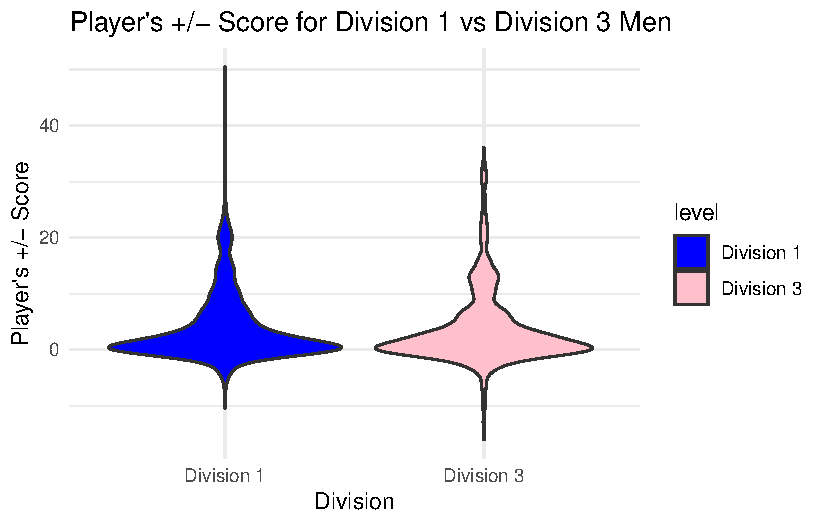
\includegraphics{final_eda_files/figure-pdf/division-level-&-plus-minus-3.pdf}

\begin{Shaded}
\begin{Highlighting}[]
\CommentTok{\# Plot a player\textquotesingle{}s plus{-}minus score and their points per game for the different divisions and genders}
\NormalTok{ultimate\_data }\SpecialCharTok{\%\textgreater{}\%} \FunctionTok{ggplot}\NormalTok{(}\FunctionTok{aes}\NormalTok{(}\AttributeTok{x =}\NormalTok{ pts\_per\_game, }\AttributeTok{y =}\NormalTok{ plus\_minus, }\AttributeTok{color =}\NormalTok{ division)) }\SpecialCharTok{+} 
   \FunctionTok{geom\_point}\NormalTok{() }\SpecialCharTok{+} \FunctionTok{geom\_smooth}\NormalTok{(}\AttributeTok{method =} \StringTok{\textquotesingle{}lm\textquotesingle{}}\NormalTok{, }\AttributeTok{se =}\NormalTok{ F) }\SpecialCharTok{+} \FunctionTok{scale\_x\_log10}\NormalTok{() }\SpecialCharTok{+}
  \FunctionTok{labs}\NormalTok{(}\AttributeTok{x =} \StringTok{"Points per game"}\NormalTok{, }\AttributeTok{y =} \StringTok{"Plus/Minus"}\NormalTok{, }\AttributeTok{color =} \StringTok{"Division"}\NormalTok{) }\SpecialCharTok{+} 
  \FunctionTok{theme\_minimal}\NormalTok{() }\SpecialCharTok{+}
  \FunctionTok{scale\_color\_viridis\_d}\NormalTok{()}
\end{Highlighting}
\end{Shaded}

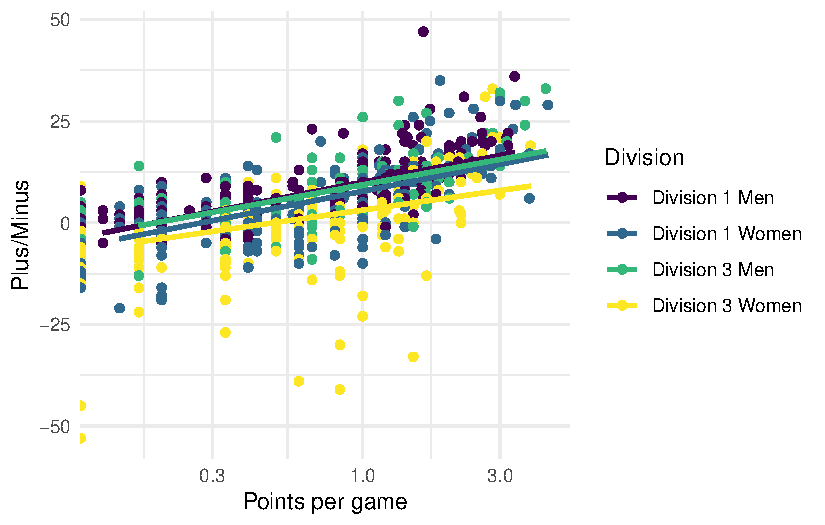
\includegraphics{final_eda_files/figure-pdf/plus-minus-&-other-variable-1.pdf}

\begin{Shaded}
\begin{Highlighting}[]
\CommentTok{\# Plot a player\textquotesingle{}s plus{-}minus score and their D\textquotesingle{}s per game for the different divisions and genders}
\NormalTok{ultimate\_data }\SpecialCharTok{\%\textgreater{}\%} \FunctionTok{ggplot}\NormalTok{(}\FunctionTok{aes}\NormalTok{(}\AttributeTok{x =}\NormalTok{ ds\_per\_game, }\AttributeTok{y =}\NormalTok{ plus\_minus, }\AttributeTok{color =}\NormalTok{ division)) }\SpecialCharTok{+} 
   \FunctionTok{geom\_point}\NormalTok{() }\SpecialCharTok{+} \FunctionTok{geom\_smooth}\NormalTok{(}\AttributeTok{method =} \StringTok{\textquotesingle{}lm\textquotesingle{}}\NormalTok{, }\AttributeTok{se =}\NormalTok{ F)}\SpecialCharTok{+}
  \FunctionTok{theme\_minimal}\NormalTok{() }\SpecialCharTok{+} \FunctionTok{scale\_x\_log10}\NormalTok{() }\SpecialCharTok{+} 
  \FunctionTok{labs}\NormalTok{(}\AttributeTok{x =} \StringTok{"Ds per game"}\NormalTok{, }\AttributeTok{y =} \StringTok{"Plus/Minus"}\NormalTok{, }\AttributeTok{color =} \StringTok{"Division"}\NormalTok{) }\SpecialCharTok{+}
  \FunctionTok{scale\_color\_viridis\_d}\NormalTok{()}
\end{Highlighting}
\end{Shaded}

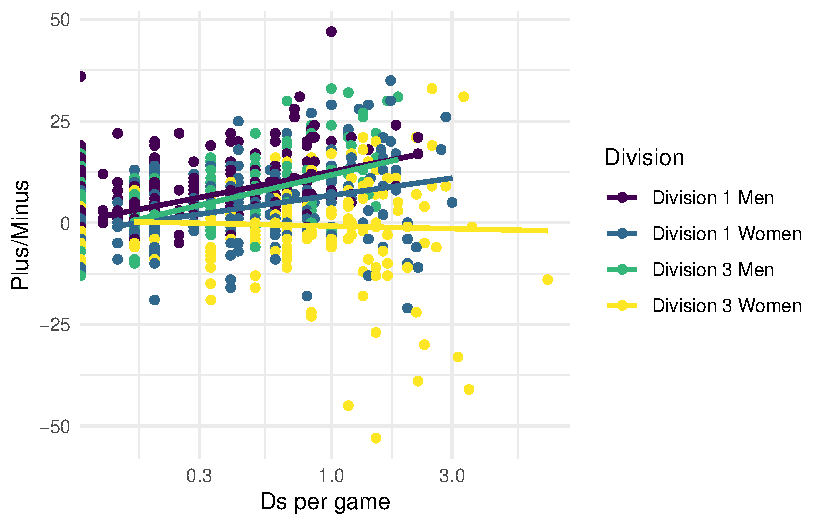
\includegraphics{final_eda_files/figure-pdf/plus-minus-&-other-variable-2.pdf}

\begin{Shaded}
\begin{Highlighting}[]
\CommentTok{\# Plot a player\textquotesingle{}s plus{-}minus score and their turns per game for the different divisions and genders}
\NormalTok{ultimate\_data }\SpecialCharTok{\%\textgreater{}\%} \FunctionTok{ggplot}\NormalTok{(}\FunctionTok{aes}\NormalTok{(}\AttributeTok{x =}\NormalTok{ turns\_per\_game, }\AttributeTok{y =}\NormalTok{ plus\_minus, }\AttributeTok{color =}\NormalTok{ division)) }\SpecialCharTok{+} 
   \FunctionTok{geom\_point}\NormalTok{() }\SpecialCharTok{+} \FunctionTok{geom\_smooth}\NormalTok{(}\AttributeTok{method =} \StringTok{\textquotesingle{}lm\textquotesingle{}}\NormalTok{, }\AttributeTok{se =}\NormalTok{ F) }\SpecialCharTok{+} \FunctionTok{scale\_x\_log10}\NormalTok{() }\SpecialCharTok{+}
  \FunctionTok{labs}\NormalTok{(}\AttributeTok{x =} \StringTok{"Turns per game"}\NormalTok{, }\AttributeTok{y =} \StringTok{"Plus/Minus"}\NormalTok{, }\AttributeTok{color =} \StringTok{"Division"}\NormalTok{) }\SpecialCharTok{+} \FunctionTok{theme\_minimal}\NormalTok{() }\SpecialCharTok{+}
  \FunctionTok{scale\_color\_viridis\_d}\NormalTok{()}
\end{Highlighting}
\end{Shaded}

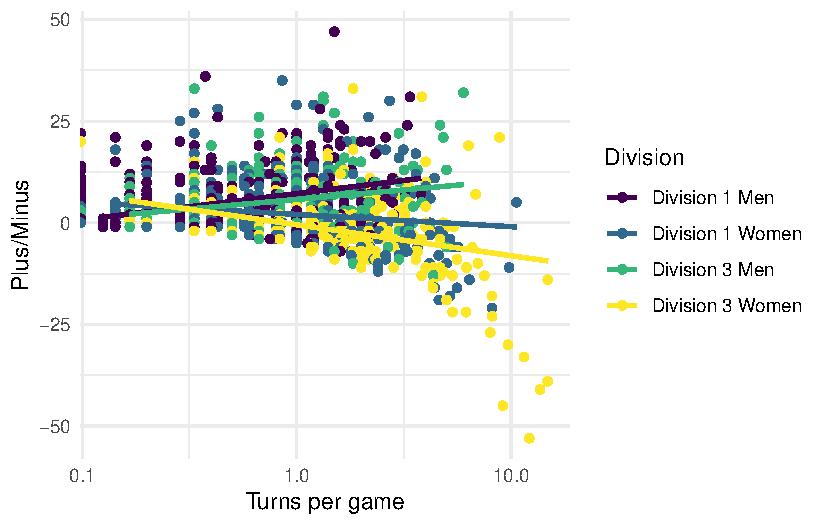
\includegraphics{final_eda_files/figure-pdf/plus-minus-&-other-variable-3.pdf}

\begin{Shaded}
\begin{Highlighting}[]
\CommentTok{\# Plot a player\textquotesingle{}s plus{-}minus score and their assists per game for the different divisions and genders}
\NormalTok{ultimate\_data }\SpecialCharTok{\%\textgreater{}\%} \FunctionTok{ggplot}\NormalTok{(}\FunctionTok{aes}\NormalTok{(}\AttributeTok{x =}\NormalTok{ ast\_per\_game, }\AttributeTok{y =}\NormalTok{ plus\_minus, }\AttributeTok{color =}\NormalTok{ division)) }\SpecialCharTok{+} 
   \FunctionTok{geom\_point}\NormalTok{() }\SpecialCharTok{+} \FunctionTok{geom\_smooth}\NormalTok{(}\AttributeTok{method =} \StringTok{\textquotesingle{}lm\textquotesingle{}}\NormalTok{, }\AttributeTok{se =}\NormalTok{ F) }\SpecialCharTok{+} \FunctionTok{scale\_x\_log10}\NormalTok{() }\SpecialCharTok{+}
  \FunctionTok{labs}\NormalTok{(}\AttributeTok{x =} \StringTok{"Assists per game"}\NormalTok{, }\AttributeTok{y =} \StringTok{"Plus/Minus"}\NormalTok{, }\AttributeTok{color =} \StringTok{"Division"}\NormalTok{) }\SpecialCharTok{+} \FunctionTok{theme\_minimal}\NormalTok{() }\SpecialCharTok{+}
  \FunctionTok{scale\_color\_viridis\_d}\NormalTok{()}
\end{Highlighting}
\end{Shaded}

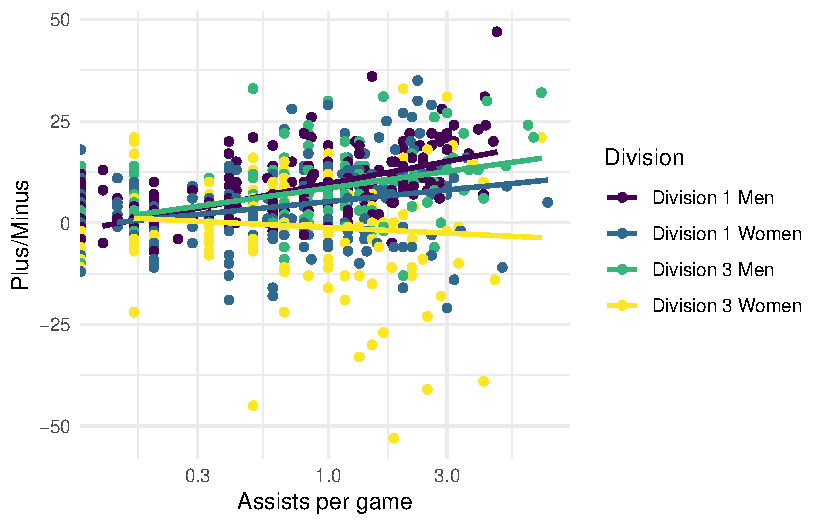
\includegraphics{final_eda_files/figure-pdf/plus-minus-&-other-variable-4.pdf}

\begin{Shaded}
\begin{Highlighting}[]
\CommentTok{\# Create a dataset df1 by selecting the following the columns below}
\NormalTok{df1 }\OtherTok{\textless{}{-}}\NormalTok{ ultimate\_data }\SpecialCharTok{\%\textgreater{}\%} \FunctionTok{select}\NormalTok{(}\FunctionTok{c}\NormalTok{(}
\NormalTok{  turns\_per\_game, ds\_per\_game, pts\_per\_game, pls\_mns\_per\_game, ast\_per\_game}
\NormalTok{))}

\CommentTok{\# Perform principle component analysis on df1 }
\NormalTok{pca }\OtherTok{\textless{}{-}}\NormalTok{ (}\FunctionTok{princomp}\NormalTok{(df1))}

\CommentTok{\# Plots the three clusters}
\FunctionTok{autoplot}\NormalTok{(}\FunctionTok{pam}\NormalTok{(df1[}\SpecialCharTok{{-}}\DecValTok{4}\NormalTok{], }\DecValTok{3}\NormalTok{), }\AttributeTok{frame =} \ConstantTok{TRUE}\NormalTok{) }\SpecialCharTok{+} \FunctionTok{theme\_minimal}\NormalTok{() }\SpecialCharTok{+}
  \FunctionTok{labs}\NormalTok{(}\AttributeTok{frame =} \StringTok{"Cluster"}\NormalTok{, }\AttributeTok{title =} \StringTok{"Principal component analysis of Ultimate data"}\NormalTok{)}
\end{Highlighting}
\end{Shaded}

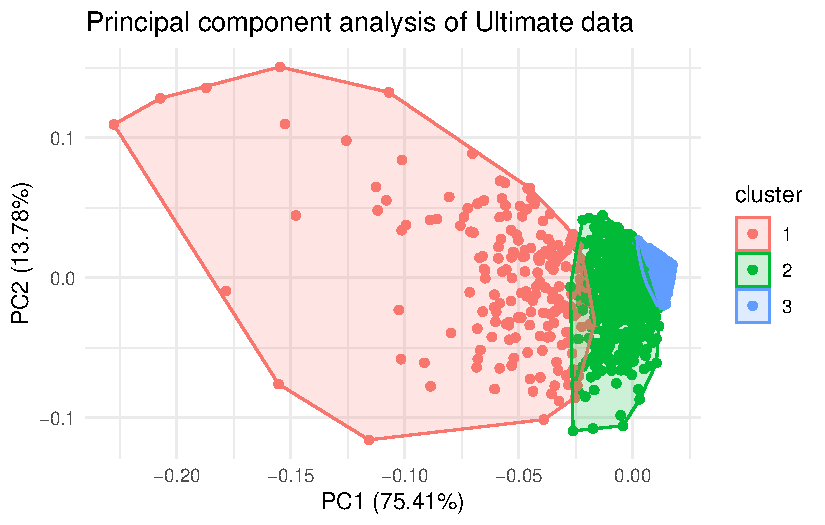
\includegraphics{final_eda_files/figure-pdf/PCA-1.pdf}



\end{document}
